\documentclass[tikz]{standalone}
\begin{document}
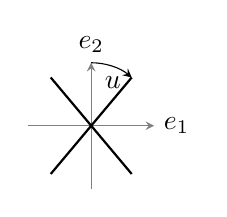
\begin{tikzpicture}[scale=.8]
\draw[-stealth,gray] (-1,0) -- (1,0) node[right,black]{\(e_1\)};
\draw[-stealth,gray] (0,-1) -- (0,1) node[above,black] {\(e_2\)};
\draw[black,thick] ({cos(180+50)},{sin(180+50)}) -- ({cos(50)},{sin(50)});
\draw[black,thick] ({cos(180-50)},{sin(180-50)}) -- ({cos(-50)},{sin(-50)});
\draw[-stealth,black] (0,1) arc (90:50:1) node[midway,below,black] {\(u\)}; 
\end{tikzpicture}
\end{document}
